\documentclass[11pt]{article}
\usepackage[margin=1in]{geometry}
\usepackage{amsmath,amssymb,amsthm,mathtools}
\usepackage{microtype}
\usepackage{graphicx}
\usepackage{booktabs}
\usepackage{placeins}
\usepackage{enumitem}
\usepackage[hidelinks]{hyperref}

\newtheorem{theorem}{Theorem}
\newtheorem{lemma}[theorem]{Lemma}
\newtheorem{proposition}[theorem]{Proposition}
\newtheorem{corollary}[theorem]{Corollary}
\newtheorem{remark}[theorem]{Remark}
\newtheorem{definition}[theorem]{Definition}

\newcommand{\E}{\mathbb{E}}
\newcommand{\Prb}{\mathbb{P}}
\newcommand{\BRF}{\textsc{BRF}}
\newcommand{\Bin}{\operatorname{Bin}}
\newcommand{\A}{\mathsf{ACTIVE}}
\newcommand{\I}{\mathsf{IDLE}}

\title{\textbf{Size Knowledge Accelerates One-Bit Las Vegas Broadcast\\
in Anonymous Dynamic Networks}}
\author{Ryutaro Yonezu\\Independent Researcher}
\date{September 8, 2026\\\small Preprint draft --- not peer reviewed}

\begin{document}
\maketitle

\begin{abstract}
We study the running-time value of network-size knowledge for a two-state
private-coin protocol for idle-start stabilizing broadcast in anonymous,
port-indistinguishable, synchronous, 1-interval-connected dynamic networks.
For Bernoulli Reactivation Flooding (BRF), an active node broadcasts and
survives independently with probability $p$, while an idle node becomes active
after receiving the broadcast.  Fair-coin BRF requires no knowledge of $n$ but
has adaptive worst-case expected stabilization time $2^{\Theta(n^2)}$.
We show that when $n$ is known, the same two persistent protocol states suffice
for expected time $2^{\Theta(n\log n)}$: it is enough to choose a size-aware
drop probability $\delta_n=2^{-k_n}$, where
$k_n=\lceil \log_2((n+1)/2)\rceil$.  The bias is implementable from fair private
coins without additional persistent protocol state.  We also prove that for
every fixed survival probability $p\in(0,1)$, a causal state-adaptive topology
adversary maximizes the Bellman continuation value by exposing exactly one idle
frontier node whenever the active set is a proper subset of the network.
Finally, we prove that $2^{\Theta(n\log n)}$ is asymptotically optimal over the
homogeneous fixed-bias BRF family against causal state-adaptive adversaries.
The optimality statement is only for this BRF family; it is not a lower bound
for all two-state randomized broadcast protocols.
\end{abstract}

\noindent\textbf{Keywords.} anonymous dynamic networks; randomized broadcast; stabilizing termination; local memory; size knowledge; Bellman equations; adversarial dynamic networks.

\section{Introduction}
Broadcast with very small persistent local memory is sharply constrained by anonymity and adversarial topology changes.  In anonymous synchronous 1-interval-connected dynamic networks, Parzych and Daymude proved that deterministic idle-start broadcast with stabilizing termination requires superconstant local memory, while their Countdown algorithm uses $O(\log n)$ memory~\cite{parzych2024}.  Turau subsequently obtained a randomized $O(\log\log n)$-space algorithm with high-probability guarantees when $n$ is known, but in the non-idle-start regime~\cite{turau2026}.  These results leave open how far private randomness can compress persistent state under the stricter idle-start requirement, and what global knowledge can buy once the state budget has already collapsed to a constant.

Our direct predecessor introduced Bernoulli Reactivation Flooding (BRF), a two-state idle-start randomized protocol with zero error, almost-sure stabilizing termination, and finite expected stabilization time for every fixed bias $p\in(0,1)$~\cite{yonezu2026brf}.  For the fair-coin choice $p=1/2$, the causal state-adaptive worst-case expectation is $2^{\Theta(n^2)}$.  Thus randomness removes the deterministic idle-start memory barrier in this protocol, but the most elementary bias pays an enormous time price.

This paper asks a narrower question: \emph{if the network size $n$ is known, can that knowledge accelerate the same two-state protocol without adding persistent protocol state?}  The answer is yes.  Choosing a drop probability on the order of $1/n$ reduces the worst-case expected time from the fair-coin $2^{\Theta(n^2)}$ scale to $2^{\Theta(n\log n)}$.  Moreover, this order is optimal within the entire homogeneous fixed-bias BRF family against causal state-adaptive topology adversaries.

\paragraph{Contributions.}
\begin{enumerate}[leftmargin=1.8em]
  \item We give a dyadic size-aware BRF bias $\delta_n=2^{-k_n}$ with $k_n=\lceil\log_2((n+1)/2)\rceil$.  It keeps exactly two persistent protocol states and satisfies
  \[
    2^{n k_n}\le W_n(p_n)\le n e^n 2^{n k_n},
  \]
  hence $W_n(p_n)=2^{\Theta(n\log n)}$.
  \item For every fixed $p\in(0,1)$, we prove that the causal state-adaptive adversary maximizes the Bellman continuation value by exposing exactly one idle frontier node whenever the active set is a proper subset of the network.
  \item We prove the fixed-bias minimax law
  \[
    \inf_{p\in(0,1)}W_n(p)=2^{\Theta(n\log n)}.
  \]
  This is a family-specific result, not a lower bound for all two-state randomized broadcast protocols.
  \item We provide reproducible exact-rational Bellman evaluations for rational biases and high-precision numerical bias optimization for $2\le n\le20$.  The experiments reproduce the predecessor's exact fair-coin values and show that the finite-size runtime optimum lies very close to the bias maximizing the uniform block-success certificate.
\end{enumerate}

\section{Related work and scope}
Parzych and Daymude study anonymous, synchronous, 1-interval-connected dynamic broadcast without identifiers or port labels.  For idle-start stabilizing termination they prove a deterministic $\omega(1)$ memory lower bound and give the $O(\log n)$-space Countdown algorithm~\cite{parzych2024}.  Our result does not contradict that lower bound because BRF is randomized; our state claim is an upper bound for persistent protocol control state under private randomness.

Turau studies randomized broadcast in the same broad anonymous dynamic setting and obtains an $O(\log\log n)$-space, constant-message algorithm with high-probability stabilization when $n$ is known~\cite{turau2026}.  That algorithm is explicitly non-idle-start: uninformed nodes may transmit before receiving the broadcast.  The present paper instead keeps the idle-start restriction and asks only how size knowledge changes the running time of a particular two-state Las Vegas protocol family.

Randomized flooding also appears in static port-aware models.  Austin, Gadouleau, Mertzios, and Trehan define Random Flooding as a randomized relaxation of Amnesiac Flooding~\cite{austin2025}.  Their nodes act per neighbor in a fixed graph, whereas our model is port-indistinguishable local broadcast on an adversarially changing connected topology.  We therefore make no generic novelty claim for randomized flooding as a mechanism.

Blanc, Di Luna, and Viglietta study deterministic computation in anonymous dynamic networks with one-bit \emph{messages}~\cite{blanc2026}.  Their one-bit resource is communication width, while the resource counted here is persistent local protocol state.  These notions should not be conflated.

Finally, the fair-coin BRF analysis and its $2^{\Theta(n^2)}$ causal state-adaptive worst-case runtime come from the direct predecessor~\cite{yonezu2026brf}.  The new claims here are the size-aware runtime improvement, arbitrary-bias one-frontier Bellman optimality, and the fixed-bias BRF-family minimax characterization.

\section{Model and protocol family}

We use the anonymous, synchronous, port-indistinguishable local-broadcast model
on a fixed node set $V$, $|V|=n\ge2$, with a connected communication graph in
every round.  There is a unique broadcaster.  The task is idle-start broadcast
with stabilizing termination, not termination detection.

A node has one persistent protocol bit, with states $\A$ and $\I$.
Initially only the broadcaster is active.  In every round, every active node
broadcasts $\mathsf{INF}$.  An active node independently remains active with
probability $p$ and becomes idle with probability
\[
  \delta:=1-p.
\]
An idle node becomes active in the next round iff it received at least one
copy of $\mathsf{INF}$ in the current round.  Active nodes do not renew their
active state in response to received copies of $\mathsf{INF}$.

We count only persistent protocol control state.  The known value $n$ is a
read-only problem parameter and is not charged to the protocol-state count.
The theorems below are stated directly for a randomized transition kernel with
survival probability $p$.  If the local random source is restricted to fair
private coins and atomic local computation is free, the dyadic bias used below
can equivalently be sampled from a finite prefix of the private coin tape
within one round.  No such transient random bits are retained across rounds.

\begin{lemma}[No false extinction]
Let $S_t$ be the active set at the start of round $t$.  If
$\varnothing\neq S_t\neq V$, then $S_{t+1}\neq\varnothing$
deterministically.  Hence a nonempty proper active set cannot jump directly to
$\varnothing$.  In particular, on the first transition into the absorbing
empty state, the preceding active set must be all of $V$; therefore every node
has already been informed before absorption.
\end{lemma}

\begin{proof}
If $S_t$ is a nonempty proper subset of $V$, connectivity of the current
snapshot gives an edge from an active node to an idle node.  The active
endpoint broadcasts $\mathsf{INF}$, so the idle endpoint is active in the next
round regardless of all survival coins.  Thus a nonempty proper active set
cannot become empty.  Now consider the first time $t+1$ for which
$S_{t+1}=\varnothing$.  By firstness, $S_t\neq\varnothing$; the preceding
argument excludes $S_t$ being a proper subset of $V$, so $S_t=V$.  Once the
active set is empty, nobody broadcasts and no idle node can reactivate, so the
empty state is absorbing.
\end{proof}

For a fixed $n$ and fixed bias $p$, let $W_n(p)$ denote the supremum of the
expected stabilization time over causal state-adaptive
1-interval-connectivity adversaries.

\section{Size-aware dyadic bias}

Define
\[
  k_n:=\left\lceil \log_2\frac{n+1}{2}\right\rceil,
  \qquad
  \delta_n:=2^{-k_n},
  \qquad
  p_n:=1-\delta_n.
\]
Then
\[
  \frac1{n+1}<\delta_n\le \frac2{n+1}.
\]
Under the fair-coin realization just described, an active node becomes idle
iff its first $k_n$ fair coin flips are all zero.  The flips may stop at the
first one, so the expected number of fair random bits consumed by an active
update is
\[
  \sum_{i=1}^{k_n}2^{-(i-1)}<2,
\]
while the worst-case number is $k_n=O(\log n)$.  This sampling procedure does
not add persistent protocol states.

\begin{lemma}[Uniform block success]
For every $p\in(0,1)$, every execution history ending in a nonempty active set,
and every causal continuation of connected snapshots, BRF reaches the
absorbing all-idle state within the next $n$ rounds with conditional
probability at least
\[
  q_n(p):=p^{n(n-1)/2}{(1-p)}^n.
\]
Consequently,
\[
  W_n(p)\le \frac{n}{q_n(p)}.
\]
\end{lemma}

\begin{proof}
Consider the event that until the active set first becomes all of $V$, every
currently active node survives, and then all $n$ active nodes drop
simultaneously.  While the active set is a nonempty proper subset, connectivity
forces at least one idle node to receive $\mathsf{INF}$.  On the chosen event
the active set therefore grows strictly until it reaches $V$, in at most
$n-1$ rounds.  The total number of required survival outcomes is at most
$1+\cdots+(n-1)=n(n-1)/2$, followed by $n$ simultaneous drop outcomes.
Thus the event has conditional probability at least $q_n(p)$ and finishes
within $n$ rounds.  Repeating the argument in $n$-round blocks gives a
geometric tail bound and the displayed expectation bound.
\end{proof}

\begin{lemma}[Universal simultaneous-drop lower bound]
For every $p\in(0,1)$, every causal topology adversary, and
$\delta=1-p$,
\[
  \E[T]\ge \delta^{-n}.
\]
\end{lemma}

\begin{proof}
The first transition into the absorbing empty state can occur only from a
round that starts with all $n$ nodes active, and then only if all $n$ nodes
independently drop.  Hence, conditioned on any nonabsorbed history, the
probability of absorption in the next round is at most $\delta^n$.  Inductively,
\[
  \Prb[T>t]\ge {(1-\delta^n)}^t.
\]
Summing the tail yields
\[
  \E[T]\ge \sum_{t\ge0}{(1-\delta^n)}^t=\delta^{-n}.
\]
\end{proof}

\begin{theorem}[Known-size one-bit runtime]
For the dyadic size-aware bias above,
\[
  2^{n k_n}
  \le
  W_n(p_n)
  \le
  n e^n 2^{n k_n}.
\]
Therefore
\[
  \log_2 W_n(p_n)
  =
  n\log_2 n+O(n),
\]
and hence
\[
  W_n(p_n)=2^{\Theta(n\log n)}.
\]
\end{theorem}

\begin{proof}
The lower bound follows from the previous lemma because
$\delta_n^{-n}=2^{nk_n}$.

For the upper bound,
\[
  W_n(p_n)
  \le
  n\,p_n^{-n(n-1)/2}\delta_n^{-n}.
\]
Since $\delta_n\le2/(n+1)$,
\[
  -\log p_n
  =
  -\log(1-\delta_n)
  \le
  \frac{\delta_n}{1-\delta_n}
  \le
  \frac{2}{n-1}.
\]
Therefore
\[
  p_n^{-n(n-1)/2}\le e^n,
\]
which gives
\[
  W_n(p_n)\le n e^n 2^{nk_n}.
\]
Finally,
$k_n=\log_2 n+O(1)$.
\end{proof}


\paragraph{Certificate-optimal continuous bias.}
The uniform $n$-round success certificate in Lemma~2 is
\[
  q_n(p)=p^{a_n}{(1-p)}^n,
  \qquad a_n:=\frac{n(n-1)}2.
\]
Maximizing $\log q_n(p)=a_n\log p+n\log(1-p)$ gives
\[
  \frac{a_n}{p}-\frac{n}{1-p}=0,
\]
and therefore the unique certificate maximizer is
\[
  p_n^{\star}=\frac{n-1}{n+1},
  \qquad
  \delta_n^{\star}=\frac{2}{n+1}.
\]
This optimizes only the uniform block-success certificate, not the actual expected stabilization time.  The dyadic choice satisfies
\[
  \frac{\delta_n^{\star}}2 < \delta_n\le\delta_n^{\star},
\]
so it is a fair-coin-implementable discretization within a factor two in drop probability.

\section{General-bias adaptive Bellman structure}

Suppose the current active-set size is $k<n$.  A state-adaptive connected
topology can expose exactly $b$ idle nodes to the active set, where
$1\le b\le n-k$.  Those $b$ idle nodes are deterministically active next
round, while each of the $k$ current active nodes independently survives with
probability $p$.  Thus
\[
  K_{t+1}=b+\Bin(k,p).
\]

Consider the one-frontier policy $b=1$, and let $\widehat E_k$ be its expected
remaining stabilization time from $k$ active nodes.  Define
\[
  \Delta_k:=\widehat E_k-\widehat E_{k+1},
  \qquad 1\le k<n.
\]

\begin{lemma}[General-bias difference recurrence]
For every $1\le k<n$,
\[
  p^k\Delta_k
  =
  1+
  \sum_{r=1}^{k-1}
  \Delta_r\,
  \Prb[\Bin(k,p)\le r-1].
\]
In particular,
\[
  \Delta_k>0
\]
for every $1\le k<n$.
\end{lemma}

\begin{proof}
Under one-frontier exposure,
\[
  \widehat E_k
  =
  1+
  \sum_{j=0}^{k}
  \binom{k}{j}p^j{(1-p)}^{k-j}\widehat E_{j+1}.
\]
For $0\le j\le k$,
\[
  \widehat E_{j+1}
  =
  \widehat E_{k+1}
  +
  \sum_{r=j+1}^{k}\Delta_r.
\]
Substitution gives
\[
  \Delta_k
  =
  1+
  \sum_{r=1}^{k}
  \Delta_r\,\Prb[\Bin(k,p)\le r-1].
\]
The $r=k$ probability equals $1-p^k$.  Moving that term to the left gives
\[
  p^k\Delta_k
  =
  1+
  \sum_{r=1}^{k-1}
  \Delta_r\,\Prb[\Bin(k,p)\le r-1].
\]
For $k=1$, this gives $\Delta_1=p^{-1}>0$.  Induction now yields
$\Delta_k>0$ for every $k<n$.
\end{proof}

\begin{theorem}[One-frontier Bellman optimality for arbitrary bias]
For every fixed $p\in(0,1)$, among all causal state-adaptive choices of
frontier size $b$ at a nonterminal state $k<n$, the Bellman-optimal choice is
\[
  b=1.
\]
\end{theorem}

\begin{proof}
The previous lemma gives
\[
  \widehat E_1>\widehat E_2>\cdots>\widehat E_n.
\]
For any realization $j$ of $\Bin(k,p)$ and any feasible $b\ge1$,
\[
  \widehat E_{1+j}\ge \widehat E_{b+j}.
\]
Hence, for every nonterminal state $k<n$,
\[
  \widehat E_k
  =
  1+\E[\widehat E_{1+\Bin(k,p)}]
  \ge
  1+\E[\widehat E_{b+\Bin(k,p)}].
\]
At $k=n$ the topology has no effect on the next active-set size, so the same
value function satisfies the unique boundary transition there, with
$\widehat E_0=0$.

This is a truncation-based verification argument.  By the uniform
block-success lemma, every admissible policy has finite expected absorption
time; in particular the one-frontier values $\widehat E_j$ are finite for all
$j$.  Fix any admissible causal state-adaptive policy $\pi$ and let $T$ be its
absorption time.  Conditional on the history at time $t<T$, apply the displayed
inequality to the policy's current feasible choice of $b$.  Equivalently,
\[
  1+\E_\pi[\widehat E_{K_{t+1}}\mid\mathcal F_t]
  \le \widehat E_{K_t}.
\]
Thus the stopped process
\[
  Z_t:=\widehat E_{K_{t\wedge T}}+(t\wedge T)
\]
is an integrable supermartingale.  For the bounded stopping time $T\wedge m$,
optional stopping gives
\[
  \E_\pi[T\wedge m]
  +\E_\pi[\widehat E_{K_{T\wedge m}}]
  \le \widehat E_k.
\]
Because $\widehat E_0=0$ and $\widehat E_j\ge0$, this implies
$\E_\pi[T\wedge m]\le\widehat E_k$ for every $m$.  Monotone convergence
then yields $\E_\pi[T]\le\widehat E_k$.  The one-frontier policy attains
equality in the Bellman relation at every nonterminal state, so its value is
exactly $\widehat E_k$ and it is Bellman-optimal.
\end{proof}

\section{Optimality within homogeneous fixed-bias BRF}

We now prove only a family-specific result.  It does not apply to arbitrary
two-state randomized broadcast protocols.

\begin{lemma}[Stopped coupling with the immigration--survival chain]
Fix $p\in(0,1)$ and let the topology adversary use one-frontier exposure
whenever the active set is a proper subset of $V$.  Let
\[
  \tau_n:=\inf\{t:K_t=n\}.
\]
Define an unrestricted auxiliary chain by
\[
  Y_0=1,
  \qquad
  Y_{t+1}=1+\Bin(Y_t,p),
\]
using fresh independent survival coins.

There exists a coupling such that the stopped processes agree pathwise:
\[
  K_{t\wedge\tau_n}
  =
  Y_{t\wedge\sigma_n}
  \qquad\text{for all }t,
\]
where
\[
  \sigma_n:=\inf\{t:Y_t=n\}.
\]
In particular,
\[
  \tau_n=\sigma_n
\]
under the coupling.

Moreover, for each fixed $t$,
\[
  Y_t
  \overset{d}{=}
  1+\sum_{r=1}^{t}B_{t,r},
\]
where $B_{t,1},\ldots,B_{t,t}$ are mutually independent and
\[
  B_{t,r}\sim\operatorname{Bernoulli}(p^r).
\]
(No joint independence across different values of $t$ is asserted or needed.)
Thus, with $X_t:=Y_t-1$,
\[
  \mu_t:=\E[X_t]
  =
  \sum_{r=1}^{t}p^r
  <
  \frac{p}{1-p}
  <
  \frac1{1-p}.
\]
\end{lemma}

\begin{proof}
Below $n$, the real one-frontier chain and the auxiliary chain have the same
transition law,
\[
  k\mapsto 1+\Bin(k,p).
\]
Couple them by using the same survival coin for each currently active
individual and the same newly exposed frontier individual.  If the two chains
agree at a state $k<n$, they therefore agree at the next state.  Also
$1+\Bin(k,p)\le k+1\le n$, so the auxiliary chain cannot jump over $n$ from a
state below $n$.  Hence the two chains agree pathwise until their common first
hit of $n$.

For the distributional representation, regard the deterministic ``$1$'' in
each update as one new immigrant.  An immigrant born $r$ rounds before time
$t$ is still present at time $t$ iff it survives $r$ independent Bernoulli-$p$
updates, which has probability $p^r$.  Distinct immigrants use disjoint
survival coins, so the indicators are independent.  Summing these indicators
gives the claimed representation and expectation.
\end{proof}

\begin{lemma}[Slow all-active hitting when the drop rate is not too small]
Let $\delta=1-p$ and suppose
\[
  \delta>n^{-1/2}.
\]
For every $n\ge3$ and every $t$,
\[
  \Prb[Y_t\ge n]
  \le
  \alpha_n
  :=
  {\left(
    \frac{e\sqrt n}{n-1}
  \right)}^{n-1}.
\]
Furthermore, for every $n\ge14$,
\[
  \E[\tau_n]
  =
  \Omega(\alpha_n^{-1})
  =
  2^{\frac12 n\log_2 n-O(n)}.
\]
\end{lemma}

\begin{proof}
By the coupling lemma,
\[
  X_t:=Y_t-1
\]
is Poisson-binomial with
\[
  \mu_t<\frac1\delta<\sqrt n.
\]
For $n\ge3$, $n-1>\sqrt n>\mu_t$, so the standard multiplicative
Poisson-binomial Chernoff bound gives
\[
  \Prb[Y_t\ge n]
  =
  \Prb[X_t\ge n-1]
  \le
  {\left(
    \frac{e\mu_t}{n-1}
  \right)}^{n-1}
  \le
  \alpha_n.
\]
Since the stopped real chain and $Y$ have the same first hit of $n$,
\[
  \Prb[\tau_n\le m]
  \le
  \sum_{t=0}^{m}\Prb[Y_t\ge n]
  \le
  (m+1)\alpha_n.
\]
For $n\ge14$,
\[
  \alpha_n\le\alpha_{14}<\frac1{16}.
\]
Indeed $e\sqrt n/(n-1)$ is decreasing in $n$ and is already below $1$ for
$n\ge10$; therefore $\alpha_n$ is decreasing from that point onward.
Take
\[
  m=\left\lfloor\frac1{8\alpha_n}\right\rfloor.
\]
Then
\[
  (m+1)\alpha_n
  \le \frac18+\alpha_n
  <\frac12,
\]
so
\[
  \Prb[\tau_n>m]>\frac12.
\]
Moreover $\alpha_n<1/16$ implies
$m\ge 1/(16\alpha_n)$.  Hence
\[
  \E[\tau_n]
  \ge
  m\,\Prb[\tau_n>m]
  \ge
  \frac1{32\alpha_n}
  =
  \Omega(\alpha_n^{-1}).
\]
Finally,
\[
  \log_2\alpha_n^{-1}
  =
  (n-1)\left(
    \log_2(n-1)
    -\frac12\log_2 n
    -\log_2 e
  \right)
  =
  \frac12 n\log_2 n-O(n).
\]
\end{proof}

\begin{theorem}[Fixed-bias BRF-family minimax order]
Let $p_n\in(0,1)$ be any size-dependent choice of homogeneous BRF survival
bias, and let
\[
  W_n(p_n)
\]
be the causal state-adaptive worst-case expected stabilization time.  Then
\[
  W_n(p_n)
  =
  2^{\Omega(n\log n)}
\]
uniformly over all such bias sequences.  Together with the dyadic size-aware
upper bound,
\[
  \inf_{p\in(0,1)} W_n(p)
  =
  2^{\Theta(n\log n)}.
\]
\end{theorem}

\begin{proof}
Write $\delta_n=1-p_n$.

If
\[
  \delta_n\le n^{-1/2},
\]
the universal simultaneous-drop lower bound gives
\[
  W_n(p_n)
  \ge
  \delta_n^{-n}
  \ge
  n^{n/2}
  =
  2^{\frac12 n\log_2 n}.
\]

If
\[
  \delta_n>n^{-1/2},
\]
choose the admissible one-frontier adversary.  Stabilization cannot occur
before the active set has hit size $n$, so
\[
  W_n(p_n)\ge \E[\tau_n].
\]
For $n\ge14$, the preceding lemma gives
\[
  W_n(p_n)
  \ge
  2^{\frac12 n\log_2 n-O(n)}.
\]
Thus every homogeneous fixed-bias BRF choice has
$2^{\Omega(n\log n)}$ state-adaptive worst-case expected time.

The size-aware dyadic choice from the first theorem satisfies
\[
  W_n(p_n)
  \le
  2^{n\log_2 n+O(n)}.
\]
Combining the two bounds proves the minimax order.
\end{proof}

\begin{remark}[Scope of the optimality claim]
The previous theorem is only an optimality result over homogeneous fixed-bias
BRF protocols: one survival probability is used by every active node in every
round for the given network size $n$.  It does not exclude faster
size-dependent protocols with additional control structure, time-varying
probabilities, history-dependent probabilities, or different two-state
randomized transition rules.
\end{remark}


\section{Computational evidence}\label{sec:experiments}
The theory above is independent of computation.  We nevertheless include finite-size Bellman calculations for three reasons: to regression-test the general-$p$ equations against the predecessor's exact fair-coin formula, to show the practical size of the knowledge-induced speedup at moderate $n$, and to compare the proof-oriented dyadic bias with biases suggested by the exact finite-state Bellman system.

\subsection{Method}
By Theorem~6, one-frontier exposure is worst-case for every fixed bias $p$.  Therefore finite worst-case expectations can be computed without enumerating graph sequences.  For states $k<n$ we solve
\[
  E_k
  =
  1+\sum_{j=0}^{k}\binom{k}{j}p^j{(1-p)}^{k-j}E_{j+1},
\]
and at the all-active state
\[
  E_n
  =
  1+\sum_{j=1}^{n}\binom{n}{j}p^j{(1-p)}^{n-j}E_j,
  \qquad E_0=0.
\]
For rational $p$, the accompanying script solves this $n\times n$ linear system with exact rational Gaussian elimination.  Fair, dyadic, and certificate-optimal biases are therefore evaluated exactly for $2\le n\le20$.  For the finite-size runtime optimum, the same Bellman system is solved at 90 decimal digits while a one-dimensional golden-section search minimizes $\log_2 E_1$ over $p\in[0.05,0.9999]$.  The numerical optimum is supporting evidence only and is not used in any theorem.

As a regression gate, exact rational evaluation at $p=1/2$ reproduces the predecessor values
\[
10,\ 58,\ 602,\ 14106,\ 755610,\ 87665306,\ 21246839962
\]
for $n=2,\ldots,8$.  The same calculation extends them to
\[
E_1(9)=10550999832730,
\qquad
E_1(10)=10622132397727898.
\]

\subsection{Finite-size comparison}
Table~\ref{tab:bias-comparison} compares the fair, dyadic, certificate-optimal, and numerically located runtime minima.  Values are reported on a base-two logarithmic scale because the expectations become enormous even at moderate $n$.

\begin{table}[ht]
\centering
\small
\begin{tabular}{r r r r r r r r}
\toprule
$n$ & $p_{\rm dy}$ & $p^\star$ & $p_{\rm num}$ & fair & dyadic & cert. & num. \\
 & & & & \multicolumn{4}{c}{$\log_2 W_n(p)$} \\
\midrule
4 & 0.7500 & 0.6000 & 0.5933 & 9.23 & 9.89 & 8.94 & 8.94 \\
6 & 0.7500 & 0.7143 & 0.7157 & 19.53 & 16.08 & 15.95 & 15.95 \\
8 & 0.8750 & 0.7778 & 0.7827 & 34.31 & 26.35 & 23.85 & 23.85 \\
10 & 0.8750 & 0.8182 & 0.8246 & 53.24 & 33.75 & 32.44 & 32.42 \\
12 & 0.8750 & 0.8462 & 0.8531 & 76.22 & 41.93 & 41.58 & 41.54 \\
16 & 0.9375 & 0.8824 & 0.8893 & 134.21 & 66.83 & 61.19 & 61.12 \\
20 & 0.9375 & 0.9048 & 0.9112 & 208.21 & 85.04 & 82.23 & 82.11 \\
\bottomrule
\end{tabular}
\caption{Finite Bellman comparison.  $p^\star=(n-1)/(n+1)$ maximizes the block-success certificate, while $p_{\rm num}$ is the high-precision minimum located by one-dimensional search on the exact Bellman expectation.}
\label{tab:bias-comparison}
\end{table}

The main pattern is robust.  Fair BRF rapidly separates from all size-aware choices.  For example, at $n=10$ the exact Bellman values give $\log_2 W_{10}(1/2)\approx53.24$, versus $33.75$ for the dyadic bias and $32.44$ for the certificate-optimal bias.  The numerically located value is $32.42$.  Thus the size-aware improvement is already large at modest $n$, while the certificate-optimal continuous bias is close to the numerical runtime optimum.

\begin{figure}[ht]
\centering
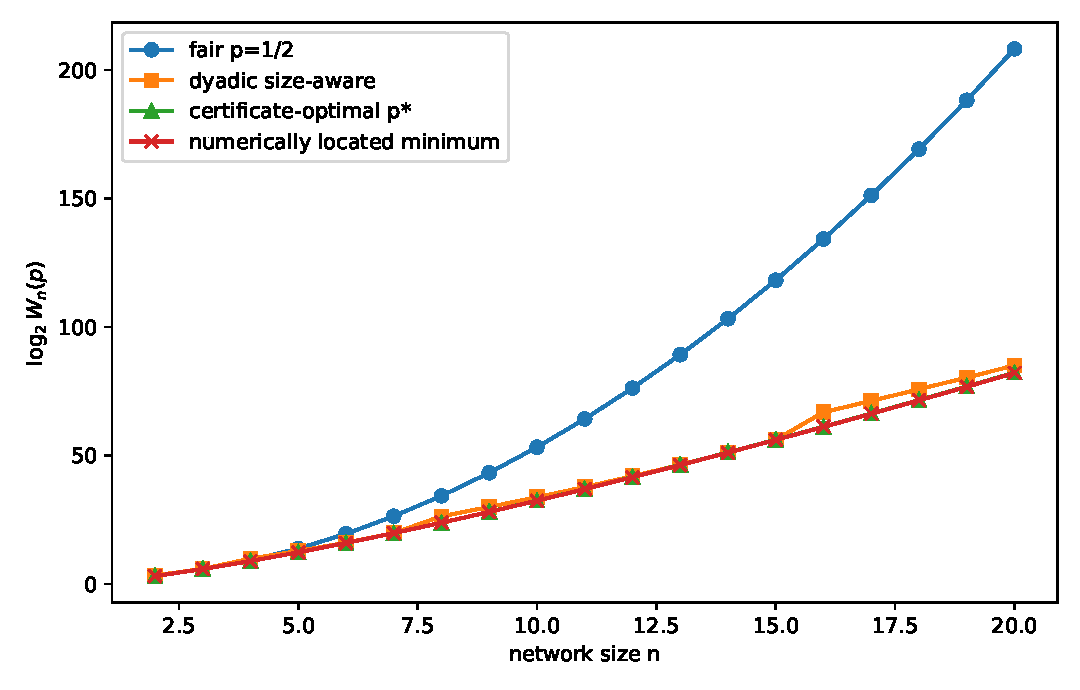
\includegraphics[width=0.88\linewidth]{figures/runtime_comparison.pdf}
\caption{Finite causal state-adaptive worst-case Bellman values.  The fair-coin curve grows on the $n^2$ exponent scale, while size-aware choices lie on the much smaller $n\log n$ scale.  The numerical curve is descriptive, not a theorem.}
\label{fig:runtime-comparison}
\end{figure}

\subsection{Bias landscape}
Figure~\ref{fig:bias-landscape} shows a sampled bias landscape at $n=10$.  The certificate maximizer $p^\star=9/11\approx0.81818$ lies close to the numerically located runtime minimum $p_{\rm num}\approx0.82458$.  The dyadic choice $p_{10}=7/8=0.875$ is deliberately constrained to a fair-coin-friendly probability and is slower at this finite size, although it has the same proved asymptotic order.

\begin{figure}[ht]
\centering
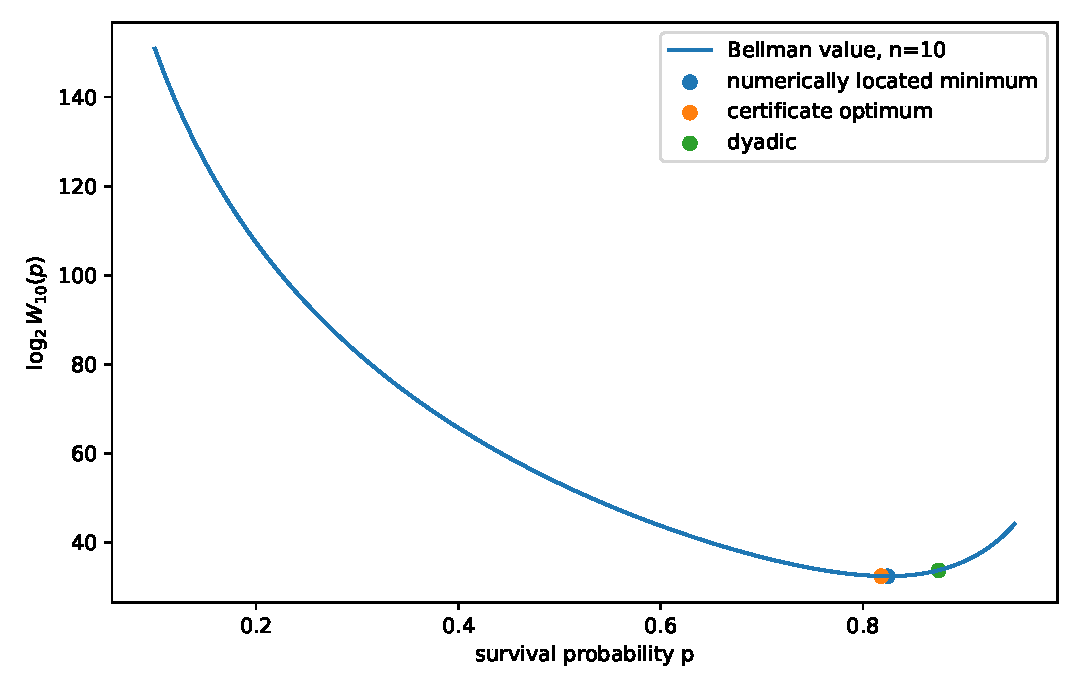
\includegraphics[width=0.88\linewidth]{figures/bias_landscape_n10.pdf}
\caption{High-precision Bellman bias landscape for $n=10$.  Markers show the numerically located runtime minimum, the block-certificate maximizer, and the dyadic size-aware choice.}
\label{fig:bias-landscape}
\end{figure}
\FloatBarrier

Across $2\le n\le20$, the certificate-optimal bias remains close to the numerically located minimum: their difference in $\log_2 W_n$ is below $0.121$ bits in the audited range.  This observation does not prove that $p^\star$ is asymptotically or exactly runtime-optimal; it only motivates the sharper open question of characterizing the true finite-$n$ optimal fixed bias.

\section{Scope, limitations, and open problems}
The safe headline claims supported by the proofs are:
\begin{enumerate}[leftmargin=1.8em]
  \item known-size dyadic BRF retains exactly two persistent protocol states and achieves $2^{\Theta(n\log n)}$ causal state-adaptive worst-case expected stabilization time;
  \item for arbitrary fixed $p\in(0,1)$, one-frontier exposure is Bellman-optimal for homogeneous \BRF{}; and
  \item $2^{\Theta(n\log n)}$ is the minimax order over homogeneous fixed-bias \BRF{}.
\end{enumerate}

The paper does \emph{not} claim that one persistent bit is the randomized minimum, that $2^{\Theta(n\log n)}$ is optimal over all two-state randomized broadcast protocols, or that either the dyadic bias or $p^\star$ exactly minimizes the actual expected stabilization time.  Time-varying biases, history-dependent randomization, and richer two-state transition kernels remain outside the lower bound.  The tight worst-case behavior against oblivious topology adversaries also remains open, as does the stronger termination-detection boundary.

\section{Conclusion}
Network-size knowledge can buy a large running-time improvement without buying additional persistent protocol state.  In BRF, fair private randomness already permits idle-start stabilizing broadcast with two persistent states, but a size-oblivious fair bias pays $2^{\Theta(n^2)}$ adaptive worst-case time.  Compiling the known size into the survival probability reduces this to $2^{\Theta(n\log n)}$, and no homogeneous fixed bias can improve that order against a causal state-adaptive adversary.  The resulting picture separates three resources that are often conflated: persistent local state, externally supplied problem knowledge, and time.

\begin{thebibliography}{10}
\small
\setlength{\itemsep}{0.25em}
\bibitem{parzych2024}
Garrett Parzych and Joshua J. Daymude.
\newblock Memory Lower Bounds and Impossibility Results for Anonymous Dynamic Broadcast.
\newblock In \emph{DISC 2024}, LIPIcs 319, Article 35, 2024.
\newblock doi:10.4230/LIPIcs.DISC.2024.35.

\bibitem{turau2026}
Volker Turau.
\newblock Broadcasts in Anonymous, Dynamic Networks: A New Algorithm and Impossibility Results.
\newblock In \emph{SAND 2026}, LIPIcs 373, Article 6, 2026.
\newblock doi:10.4230/LIPIcs.SAND.2026.6.

\bibitem{austin2025}
Henry Austin, Maximilien Gadouleau, George B. Mertzios, and Amitabh Trehan.
\newblock Amnesiac Flooding: Easy to Break, Hard to Escape.
\newblock In \emph{DISC 2025}, LIPIcs 356, Article 10, 2025.
\newblock doi:10.4230/LIPIcs.DISC.2025.10.

\bibitem{blanc2026}
Thibaut Blanc, Giuseppe Antonio Di Luna, and Giovanni Viglietta.
\newblock Computing in Anonymous Dynamic Networks with One-Bit Communications.
\newblock arXiv:2607.08358, 2026.

\bibitem{yonezu2026brf}
Ryutaro Yonezu.
\newblock Randomization Collapses the Idle-Start Memory Barrier for Anonymous Dynamic Broadcast.
\newblock Zenodo preprint, 2026.
\newblock doi:10.5281/zenodo.22643897.
\end{thebibliography}

\end{document}
